% Created 2017-10-02 Mon 10:41
% Intended LaTeX compiler: pdflatex
\documentclass[11pt]{article}
\usepackage[utf8]{inputenc}
\usepackage[T1]{fontenc}
\usepackage{graphicx}
\usepackage{grffile}
\usepackage{longtable}
\usepackage{wrapfig}
\usepackage{rotating}
\usepackage[normalem]{ulem}
\usepackage{amsmath}
\usepackage{textcomp}
\usepackage{amssymb}
\usepackage{capt-of}
\usepackage{hyperref}
\author{Johannes Brauer}
\date{\today}
\title{Parallelprogrammierung -- Einstieg}
\hypersetup{
 pdfauthor={Johannes Brauer},
 pdftitle={Parallelprogrammierung -- Einstieg},
 pdfkeywords={},
 pdfsubject={},
 pdfcreator={Emacs 25.1.1 (Org mode 9.0.9)}, 
 pdflang={Germanb}}
\begin{document}

\maketitle

\section*{Warum Parallelprogrammierung?}
\label{sec:org8d1d276}

\subsection*{Technische Gründe}
\label{sec:org0d37114}
\begin{itemize}
\item Erhöhung der Rechenleistung durch Erhöhung der Taktfrequenzen stösst
technisch an Grenzen
\item Mooresche Gesetz gilt aber noch.
\item Folge: Prozessoren mit mehreren Kernen.
\item Leistungssteigerung durch Parallelarbeit
\item Geschwindigkeitssteigerung bei \(n\) Kernen theoretisch n-fach
\begin{itemize}
\item praktisch nicht erreichbar
\item Anwendungsentwicklung auf Parallelprogrammierung nicht vorbereitet
\end{itemize}
\end{itemize}
\subsection*{Enwicklung der Mikroprozessortechnik}
\label{sec:org0e0261f}
\begin{center}
\includegraphics[width=.9\linewidth]{./Abbildungen/CPU-Moore.png}
\end{center}
\subsection*{Robert C. Martin: The failure of state}
\label{sec:org9bbb745}
\href{https://www.youtube.com/watch?v=7Zlp9rKHGD4}{Functional Programming -- The Failure of State}

Ausschnitte:
\begin{itemize}
\item 34:34 - \href{https://www.youtube.com/watch?v=7Zlp9rKHGD4\&t=2074s}{fewer concurrency issues}
\item 36:12 - Moore's law bis 43:47
\item 49:44 - \href{https://www.youtube.com/watch?v=7Zlp9rKHGD4\&t=2984s}{OO = procedure + state} bis 50:56
\item 53:57 - \href{https://www.youtube.com/watch?v=7Zlp9rKHGD4\&t=3237s}{impose  discipine on the change of state} bis 55:12
\end{itemize}

\section*{Prozesse, Threads, Synchronisation}
\label{sec:org32848d1}
(Die Ausführungen in diesem lehnen sich an ein Vorlesungsskript von
Uwe Neuhaus an)
\subsection*{Bestandteile von Computersystemen}
\label{sec:org564125a}
\begin{enumerate}
\item Hardware – Bereitstellung grundlegender Betriebsmittel (Prozessor,
Speicher, Ein-/Ausgabegeräte)
\item Betriebssystem – steuert und koordiniert die Nutzung der
Betriebsmittel für die verschiedenen Anwendungsprogramme der
verschiedenen Anwender
\item Anwendungsprogramme – definieren, wie das zu bearbeitende Problem
mit Hilfe der Betriebsmittel gelöst wird (Compiler,
Datenbanksysteme, Textverarbeitung, Spiele usw.)
\item Anwender (Menschen, Maschinen, andere Computer)
\end{enumerate}
\subsection*{Abstrakte Sicht der Bestandteile}
\label{sec:org77347f8}
\begin{center}
\includegraphics[width=.9\linewidth]{./Abbildungen/computersystem.png}
\end{center}
\subsection*{Mehrprogrammbetrieb}
\label{sec:orgd3d6f4b}
\subsubsection*{Stapelverarbeitung}
\label{sec:org5f46e13}
\begin{center}
\includegraphics[width=.9\linewidth]{./Abbildungen/mehrprogrammbetrieb.png}
\end{center} Mehrere Aufträge werden im
Speicher gehalten. Der Prozessor wechselt zwischen diesen Aufträgen
hin und her.
\subsubsection*{CPU-Aufteilung}
\label{sec:org052f4de}

\begin{nebeneinander}
Ablauf eines Programms:
\begin{center}
\includegraphics[width=.9\linewidth]{./Abbildungen/EinProgrammbetrieb.png}
\end{center}
\end{nebeneinander}

\begin{nebeneinander}
quasi-paralleler Ablauf zweier Programme:
\begin{center}
\includegraphics[width=.9\linewidth]{./Abbildungen/ZweiProgramme.png}
\end{center}
\end{nebeneinander}

\begin{clear}
\end{clear}


\subsubsection*{Benötigte Betriebssystemfähigkeiten beim Mehrprogrammbetrieb}
\label{sec:org9f633a7}
\begin{itemize}
\item Bereitstellung von Ein-/Ausgabe-Routinen
\item Zuordnung von Geräten zu   Aufträgen
\item Speicherverwaltung – das Betriebssystem muss den verschiedenen
Aufträgen Speicher zuordnen
\item Prozessor-Scheduling – das Betriebssystem muss zwischen den
verschiedenen, ausführbereiten Aufträgen auswählen
\item Schutz vor Programmfehlfunktionen (Übergriffen eines Auftrags auf
einen anderen, Endlosschleifen usw.)
\end{itemize}
\subsection*{Mehrbenutzersystem (Time-Sharing Systems) – Interaktive Benutzung}
\label{sec:org2e1055c}
\begin{itemize}
\item Eine interaktive Kommunikationsmöglichkeit zwischen dem Anwender und
der Computersystem wird bereitgestellt, die den Zugriff auf
Programme und Daten erlaubt. Nach der Abarbeitung eines Kommandos
wird das nächste Benutzerkommando erwartet.
\item Der Prozessor wird in schneller Abfolge zwischen verschiedenen
Aufträgen, die sich im Speicher und auf Festplatte befinden, hin und
her geschaltet. (Nur Aufträge im Speicher erhalten den Prozessor.)
\item Ein Auftrag wird in den Hauptspeicher ein- oder auf Festplatte
ausgelagert.
\end{itemize}
\subsection*{Arbeitsplatzrechnersysteme / Personal-Computer}
\label{sec:org8c81224}
\begin{itemize}
\item Personal-Computer – Computersysteme, die ausschließlich einem
einzigen Benutzer zur Verfügung stehen
\item Ein-/Ausgabegeräte – Tastatur, Maus, Monitor, kleiner Drucker, \ldots{}
\item Komfortable Bedienung, schnelle Reaktionszeit
\item Konzepte größerer Betriebssysteme können verwendet werden
(z.B. Time-Sharing). Andere Aspekte u.U. weniger wichtig
(z.B. Prozessor- Auslastung). Ausführung verschiedener
Betriebssysteme möglich (Windows, MacOS, UNIX, Linux)
\end{itemize}
\subsection*{Mehrprozessorsysteme}
\label{sec:org8f6d8fe}
\subsubsection*{Prinzip}
\label{sec:orgb5a3cd7}
\begin{itemize}
\item Mehrprozessorsysteme besitzen mehrere, eng gekoppelte Prozessoren
\item Eng gekoppelt -- Prozessoren nutzen gemeinsam Hauptspeicher und
Systemtakt. Die Kommunikation zwischen den Prozessoren findet
üblicherweise über den gemeinsam genutzten Speicher statt.
\item Vorteile von Mehrprozessorsystemen: Erhöhter Durchsatz
\begin{itemize}
\item Verbessertes Preis/Leistungsverhältnis
\item Höhere Zuverlässigkeit
\begin{itemize}
\item stufenweiserLeistungsverlust(gracefuldegradation) •
\item Ausfallsicherheit(fail-softsystems)
\end{itemize}
\end{itemize}
\end{itemize}
\subsubsection*{Varianten}
\label{sec:org5087024}
\begin{description}
\item[{Symmetric multiprocessing (SMP)}] \begin{itemize}
\item Auf jedem Prozessor läuft das identische Betriebssystem
\item Mehrere Prozesse können ohne Leistungsverlust ablaufen
\item Die meisten modernen Betriebssysteme unterstützen SMP
\end{itemize}
\item[{Asymmetric multiprocessing}] \begin{itemize}
\item Jeder Prozessor hat eine spezielle Aufgabe. Ein Master-Prozessor
verteilt Aufgaben an die anderen (möglicherweise spezialisierten)
 Slave- Prozessoren.
\item Beispiel: Grafikprozessoren
\end{itemize}
\end{description}
\subsubsection*{Architektur bei symmetrischen Mehrprozessorsystemen}
\label{sec:org9df2dff}
\begin{center}
\includegraphics[width=.9\linewidth]{./Abbildungen/mehrprozessorarchitektur.png}
\end{center}

\textbf{Achtung}: Zugriff auf den Hauptspeicher über gemeinsamen Bus kann zum
Flaschenhals werden.

\subsection*{Prozesse}
\label{sec:org00ceb1b}
Für die Behandlung der Anforderungen in Mehrprogrammbetriebssystemen
sind primitive Ad-hoc-Lösungen nicht mehr möglich. Das Verständnis des
Gesamtsystems ist nicht mehr durch die Beschreibung des Verhaltens der
CPU zu jedem Zeitpunkt möglich, da das Verhalten der CPU in
Mehrbenutzersystemen im Mehrprogrammbetrieb stark von nicht
vorhersagbaren externen Ereignissen (Unterbrechungen) abhängig ist. Das
Betriebssystem wird als Ansammlung von funktionellen Einheiten
betrachtet, die zunächst unabhängig voneinander arbeiten aber über
wohldefinierte Schnittstellen miteinander kommunizieren müssen. Diese
funktionellen Einheiten bezeichnet man als \textbf{Prozesse}.
\subsubsection*{Prozessbegriff}
\label{sec:orgec149ba}
\paragraph*{Typische Merkmale von Prozessen:}
\label{sec:org9886e81}
\begin{itemize}
\item brauchen Prozessor
\item enthalten jeweils ein sequentielles Programm
\item können grundsätzlich parallel ablaufen
\end{itemize}

Zur Abgrenzung zum Begriff \emph{Benutzerauftrag} (\emph{Job}): Zur Abarbeitung
eines Benutzerauftrags sind in der Regel mehrere Prozesse notwendig.

\paragraph*{Formen der Parallelität}
\label{sec:orgb4f4dd8}
\begin{itemize}
\item mehrere Prozesse laufen auf unterschiedlichen Prozessoren ab --
(tatsächlich parallel)

\item ein Prozessor wird "scheibchenweise" den Prozessen zugeordnet, sodass
diese „überlappt“ ablaufen --
(quasi-parallel)
\end{itemize}

Die im Zusammenhang mit der Parallelität von Prozessen auftretenden
Probleme sind davon aber unabhängig.
\subsection*{Synchronisation konkurrierender Prozesse}
\label{sec:org7a36ce2}
\subsubsection*{Problem des wechselseitigen Ausschlusses}
\label{sec:org62d9dad}
Das Problem des wechselseitigen Ausschlusses (\emph{mutual exclusion}) wurde
erstmals 1965 von Edsger W. Dijkstra formuliert.

\paragraph*{Beispiel 1:}
\label{sec:orgf8dab81}
Zwei zyklische Prozesse \(p_1\) und \(p_2\) benutzen von Zeit zu Zeit ein
Magnetband. Es steht nur ein Gerät zur Verfügung, das nicht von mehr als
einem Prozess gleichzeitig benutzt werden kann.

\textbf{1. Lösungsversuch:} Definition einer booleschen Variable \texttt{frei}\\
\begin{nebeneinander}
\(p_1\):
\begin{verbatim}
001 wiederhole
002 wiederhole bis frei;
003   frei := false;
004   benutze(magnetband)
005   frei := true;
... ...
FFF ständig\\
\end{verbatim}
\end{nebeneinander}
\begin{nebeneinander}
\(p_2\):
\begin{verbatim}
001 wiederhole
002 wiederhole bis frei;
003   frei := false;
004   benutze(magnetband)
005   frei := true;
... ...
FFF ständig
\end{verbatim}
\end{nebeneinander}
\begin{clear}
\end{clear}
\textbf{Probleme:} 
\begin{itemize}
\item Wenn \(p_1\) und \(p_2\) parallel ablaufen, können sie auch gleichzeitig
das Magnetband als frei erkennen. Das gleiche Problem kann auch bei
quasi-parallel ablaufenden Prozessen auftreten, da jeder Prozess
zwischen \texttt{002} und \texttt{003} unterbrochen werden kann.
\item Durch die Warteschleife wird Prozessorzeit beansprucht (\emph{busy
waiting}).
\end{itemize}
\textbf{2. Lösungsversuch:} Definition einer booleschen Variable \texttt{p1anderReihe}\\
\begin{nebeneinander}
\(p_1\):
\begin{verbatim}
001 wiederhole
002   wiederhole bis p1anderReihe;
003   benutze(magnetband)
004   p1anderReihe := false;
... ...
FFF ständig
\end{verbatim}
\end{nebeneinander}
\begin{nebeneinander}
\(p_2\):
\begin{verbatim}
001 wiederhole
002   wiederhole bis nicht p1anderReihe;
003   benutze(magnetband)
004   p1anderReihe := true;
... ...
FFF ständig
\end{verbatim}
\end{nebeneinander}
\begin{clear}
\end{clear}

Ein wechselseitiger Ausschluss ist zwar gewährleistet, allerdings müssen
die Prozesse das Magnetband abwechselnd benutzen. Beide Prozesse müssen
außerdem „am Leben” bleiben. \emph{Busy waiting} tritt auch hier auf.
\textbf{3. Lösungsversuch:} Definition zweier boolesche Variablen \texttt{p1istdran} und \texttt{p2istdran}

Initialisierung:

\begin{verbatim}
p1istdran := false
p2istdran := false
\end{verbatim}
\begin{nebeneinander}
\(p_1\):
\begin{verbatim}
wiederhole
   p1istdran := true
   wiederhole bis nicht p2istdran
   benutze(magnetband)
   p1istdran := false
...  
ständig
\end{verbatim}
\end{nebeneinander}
\begin{nebeneinander}
\(p_2\):
\begin{verbatim}
wiederhole
   p2istdran := true
   wiederhole bis nicht p1istdran
   benutze(magnetband)
   p2istdran := false
...
ständig
\end{verbatim}
\end{nebeneinander}
\begin{clear}
\end{clear}
Wechselseitiger Ausschluss ist zwar garantiert, es besteht aber die
Gefahr der Verklemmung (\emph{deadlock}).

\subsubsection*{Anforderungen an eine Lösung für das Problem des wechselseitigen Ausschlusses:}
\label{sec:org1c6da69}

\begin{enumerate}
\item Das Betriebsmittel wird nach endlicher Zeit zugewiesen.
\item Ein Prozess gibt das Betriebsmittel nach endlicher Zeit wieder frei.
\item Ein Prozess, der wartet, soll keine Rechenzeit verbrauchen.
\item Eine Problemlösung soll von den Prozessen in eine gemeinsame Umgebung
verlagert werden.
\end{enumerate}
Das grundsätzliche Problem resultiert aus der „unkontrollierten“
Benutzung gemeinsamer Betriebsmittel.

\subsubsection*{Weitere Beispiele für das Auftreten des Problems des wechselseitigen}
\label{sec:orga81e02f}
Ausschlusses:

\begin{enumerate}
\item Veränderung von Datensätzen in einer von mehreren Prozessen gemeinsam
benutzten Datei

\item gemeinsame Benutzung von Unterprogrammen mit lokalen Variablen für
Zwischenergebnisse
\end{enumerate}

\subsubsection*{Definition (kritischer Abschnitt):}
\label{sec:org8009881}
Programmabschnitte, in denen sich zu einem Zeitpunkt nur jeweils ein
Prozess befinden darf, heißen \emph{kritische Abschnitte} (\emph{critical
sections}).

\subsubsection*{Lösung: \texttt{P}- und \texttt{V}-Operationen nach Edsger W. Dijkstra}
\label{sec:orga28f678}
\texttt{P} und \texttt{V} sind zwei Operationen auf einer gemeinsamen Variablen,
genannt \emph{Semaphorvariable}. Jedem kritischen Abschnitt wird eine
Semaphore zugeordnet.

\paragraph*{Definition von \texttt{P} und \texttt{V}:}
\label{sec:org4eeac52}
\begin{verbatim}
    P(s):
       wenn s=1
       dann s:=0
       sonst blockiere den aufrufenden Prozess
             und schalte auf anderen Prozess um
        
    V(s):
       wenn ein Prozess auf s wartet
       dann loese den Prozess aus Wartezustand
       sonst s:=1
\end{verbatim}

\paragraph*{Beispiel für die Sicherung eines kritischen Abschnitts (Benutzung eines Magnetbandgeräts) \ldots{}}
\label{sec:org93e336b}
\ldots{} durch eine Semaphore \texttt{s}:

\begin{verbatim}
P(s)
benutze(magnetband)
V(s)
\end{verbatim}

\paragraph*{Eigenschaften von \texttt{P} und \texttt{V}:}
\label{sec:org67efb8d}
\begin{itemize}
\item sind selbst kritische Abschnitte
\item müssen atomar sein (dürfen nicht selbst unterbrochen werden)
\item Es handelt sich aber um \textbf{kurze} kritische Abschnitte, die im
Systemkern realisiert werden, wo wechselseitiger Ausschluss einfach zu implementieren ist.
\item Sie werden häufig mithilfe eines Spezialbefehls des Prozessors
realisiert, wobei ein aktives Warten in Kauf genommen wird.
\item Dazu wird eine Sperrvariable \texttt{pv} mit folgender Bedeutung eingeführt:
\end{itemize}

\begin{center}
\begin{tabular}{ll}
\texttt{pv=1} : & \texttt{P}- und \texttt{V}-Operationen können ausgeführt werden\\
\texttt{pv=0} : & \texttt{P}- und \texttt{V}-Operationen können nicht ausgeführt werden\\
\end{tabular}
\end{center}

\paragraph*{Der Spezialbefehl \texttt{teste\_und\_setze(pv)}}
\label{sec:org1877ef8}
\ldots{} ist eine unteilbare Operation, die folgendermaßen arbeitet:

\begin{verbatim}
   wiederhole solange pv = 0; (* tue nichts, busy waiting *)
   pv := 0
\end{verbatim}

Mithilfe dieses Befehls werden nun zwei modifizierte Operationen \texttt{P’}
und \texttt{V’} eingeführt, die dann zur Sicherung eines kritischen Abschnitts
eingesetzt werden können.

\begin{nebeneinander}
\begin{verbatim}
P'(s)
   teste_und_setze(pv)
   P(s)
   pv:=1
\end{verbatim}
\end{nebeneinander}
\begin{nebeneinander}
\begin{verbatim}
V'(s)
   teste_und_setze(pv)
   V(s)
   pv:=1
\end{verbatim}
\end{nebeneinander}
\begin{clear}
\end{clear}
\subsubsection*{Alternative Realisierung für Semaphore}
\label{sec:orgd56cd15}
\begin{itemize}
\item \texttt{S} ist ein Semaphoren-Objekt mit den Methoden \texttt{wait()} (möchte
passieren) und \texttt{signal()} (verlassen).
\item Ein Semaphoren-Objekt ist meist verbunden mit einer zugehörigen
Prozess-Warteschlange \texttt{W}.
\end{itemize}
\begin{nebeneinander}
Prozess 1
\begin{verbatim}
S.wait();
i = leseZaehler();
i = i + 10; 
schreibeZaehler( i ); 
S.signal();
\end{verbatim}
\end{nebeneinander}
\begin{nebeneinander}
Prozess 2
\begin{verbatim}
S.wait();
j = leseZaehler();
j = j - 5; 
schreibeZaehler( j ); 
S.signal();
\end{verbatim}
\end{nebeneinander}
\begin{clear}
\end{clear}
\paragraph*{Realisierung eines binären Semaphors}
\label{sec:orgd0d1363}
\begin{verbatim}
S.wait():
if ( TestAndSet(belegt) ) {
   Prozess in Warteschlange W einreihen; 
   Prozess in Zustand „wartend“ versetzen;
}
\end{verbatim}
\begin{verbatim}
S.signal():
if ( W.empty() == false ) {
   Einen Prozess aus Warteschlange W lösen; 
   Prozess in Zustand „bereit“ versetzen;
}
else { belegt = false; }
\end{verbatim}
\paragraph*{Realisierung eines Zähl-Semaphors}
\label{sec:org38b9bf2}
\begin{verbatim}
S.wait():
if ( FetchAndAdd( zaehler, -1 ) < 1) {
   Prozess in Warteschlange W einreihen; 
   Prozess in Zustand „wartend“ versetzen;
}
\end{verbatim}
\begin{verbatim}
S.signal():
if ( FetchAndAdd( zaehler, 1 ) < 0 ) {
   Einen Prozess aus Warteschlange W lösen; 
   Gelösten Prozess in Zustand „bereit“ versetzen;
}
\end{verbatim}
\subsection*{Synchronisation kooperierender Prozesse}
\label{sec:org7d0f23d}
\begin{itemize}
\item Bisher wurden nur um gemeinsame Betriebsmittel konkurrierende
Prozesse betrachtet, die sonst nichts miteinander zu tun hatten.
\item Kooperation zwischen Prozessen kann z.B. heißen, dass Nachrichten
zwischen einem Erzeuger und einem Verbraucher ausgetauscht werden
(\emph{producer-consumer-problem}).
\item Nachrichtenaustausch soll gepuffert erfolgen, um Erzeuger und
Verbraucher bezüglich ihrer Arbeitsgeschwindigkeit zu entkoppeln.
\item Ringpuffer fester Größe kann nur eine feste Anzahl von Nachrichten
speichern.
\item Abbildung zeigt einen teilweise gefüllten Ringpuffer mit zwei
Zeigern, \texttt{c} für den Verbraucher und \texttt{p} für den Erzeuger.  
\begin{center}
\includegraphics[width=.9\linewidth]{./Abbildungen/ringpuffer.png}
\end{center}

\item Beide Prozesse bearbeiten den Puffer im Uhrzeigersinn. Durch die
Prozesssynchonisation muss verhindert werden, dass sie sich
gegenseitig „überholen”.
\end{itemize}

\subsubsection*{Sychronisation von Erzeuger un Verbraucher durch Semaphore}
\label{sec:orgaffe63a}

\begin{itemize}
\item Die Prozesse benutzen jeweils eine Kommunikationsprozedur,
\texttt{SendeNachricht} und \texttt{EmpfangeNachricht}, die dafür sorgen, dass
derErzeuger wartet, wenn der Puffer voll ist, und der Verbraucher,
wenn der Puffer leer ist.
\end{itemize}


\begin{nebeneinander}
\textbf{Konsument}
\begin{verbatim}
EmpfangeNachricht(puffer)
  while (true) {
     belegt.wait();
     mutex.wait();
     nachricht = holeAusPuffer(); 
     mutex.signal();
     frei.signal();
     konsumiere(nachricht); 
  }
\end{verbatim}
\end{nebeneinander}
\begin{nebeneinander}
\textbf{Produzent}
\begin{verbatim}
SendeNachricht(puffer)
  while (true) {
     nachricht = erzeuge();
     frei.wait();
     mutex.wait();
     schreibeInPuffer(nachricht); 
     mutex.signal();
     belegt.signal();
  }
\end{verbatim}
\end{nebeneinander}
\begin{clear}
\end{clear}

Initialisierung: \texttt{mutex.zaehler = 1; frei.zaehler = max; belegt.zaehler = 0;}

\paragraph*{Nachteil dieser Lösung}
\label{sec:orge7fe319}
\begin{itemize}
\item Die Verantwortung für die korrekte Synchronisation bzw. deren
korrekte Programmierung liegt bei den Prozessen.
\item Programmierfehler können dabei zu schwer reproduzierbarem
Fehlverhalten (z.B. Verklemmungen) führen.
\end{itemize}

\subsubsection*{Weitere klassische Synchronisationsprobleme}
\label{sec:orgcc9fc33}
\begin{description}
\item[{Readers-Writers-Problem}] \begin{itemize}
\item Einige Prozesse/Threads wollen einen Datenbereich lesen, einige
wollen ihn verändern.
\item Gleichzeitiger Lesezugriff ist erlaubt.
\item Schreibzugriffe müssen exklusiv erfolgen.
\end{itemize}
\item[{Dining-Philosophers-Problem}] \begin{itemize}
\item Fünf Philosophen sitzen um einen runden Tisch, denken nach und
essen Reis mit Stäbchen.
\item Zwischen den Tellern liegt jeweils ein Stäbchen, zum Essen braucht man aber zwei.
\end{itemize}
\end{description}

\subsection*{Monitore}
\label{sec:org2fe89c8}
\begin{itemize}
\item \textbf{Programmiersprachliches} Konstrukt, funktional äquivalent zu Semaphoren
\item Kritische Methoden und Daten werden in einer Klasse mit einem
zugehörigen Semaphor kombiniert.
\item Leichter zu handhaben, weniger fehleranfällig
\item Unterstützung der Synchronisation durch \emph{Bedingungsvariablen}
\end{itemize}

\subsection*{Synchronisation durch Nachrichtenaustausch}
\label{sec:orgd66a7bd}

\begin{itemize}
\item Die bisher betrachteten Synchronisationsprimitive sind nur
einsetzbar, wenn die beteiligten Prozesse Zugriff auf einen
gemeinsamen Speicherbereich (shared memory) haben, in dem sich
z.B. die Semaphorvariablen befinden.
\item Auf diese Art ist daher die Synchronisation in Verteilten Systemen,
wo Prozesse auf unterschiedlichen Maschinen ablaufen können, nicht
möglich.
\item Hierfür werden neue Synchronisationsprimitive (Aufrufe des
Systemkerns), die auf dem Austausch von Nachrichten (\emph{message
passing}) basieren, eingeführt:

\texttt{send(destination,message)} \\
\texttt{receive(source,message)}
\end{itemize}
\begin{itemize}
\item Mit \texttt{send} und \texttt{receive} können Prozesse synchronisiert werden, die
auf Prozessoren ohne gemeinsamen Speicher ablaufen.
\item Bei einem Aufruf von \texttt{send} wird der Prozess blockiert, wenn keine
Nachricht übermittelt werden kann. Bei einem Aufruf von \texttt{receive}
wird der Prozess blockiert, wenn keine Nachricht verfügbar ist.
\end{itemize}

\subsubsection*{Mögliche Schwierigkeiten bei der Nachrichtenübermittlung:}
\label{sec:orgc797bef}

\begin{itemize}
\item Verlust einer Nachricht\\
Abhilfe: jede gesendete Nachricht muss quittiert werden
(\emph{acknowledgement}), wiederholen der Nachricht beim Ausbleiben der
Quittung
\item Verlust der Quittung
\item doppeltes Eintreffen einer Nachricht beim Empfänger\\
Abhilfe: Numerieren der Nachrichten
\item Eindeutige Benennung (Adressierung) von:
\begin{itemize}
\item Prozessoren
\item Maschinen
\item \emph{domains}
\end{itemize}
\item Sicherheitsprobleme
\item Effizienz, wenn Sender und Empfänger auf der gleichen Maschine laufen
\end{itemize}

\subsubsection*{Behandlung des \emph{Producer-Consumer-Problems} mit \emph{message passing}:}
\label{sec:org55e7e97}

Annahmen:
\begin{itemize}
\item Nachrichten haben feste Länge.
\item Gesendete, aber noch nicht empfangene Nachrichten werden vom
Betriebssystem automatisch gepuffert.
\item Maximal \texttt{max} Nachrichten können gepuffert werden.
\end{itemize}

\begin{verbatim}
    Consumer:
        for i := 1 to max do send(producer,emptymessage);
        while true do begin
           receive(producer,message);
           extract_data(message);
           send(producer,emptymessage);
           process(data);
        end

    Producer:
        while true do begin
           produce_data(data);
           receive(consumer,emptymessage);
           build_message(message,data);
           send(consumer,message);
        end
\end{verbatim}

\paragraph*{Anmerkungen:}
\label{sec:orgcd92d66}
\begin{itemize}
\item Die Zahl der Nachrichten bleibt konstant.
\item Für Pufferung ist ein fester Speicherbereich vorgesehen.
\item Pufferung und Adressierung erfolgt durch sog. \emph{mailboxes} bei Sender
und Empfänger.
\item in UNIX entsprechen sogenannte \emph{pipes} den \emph{mailboxes}.
\end{itemize}

\subsection*{Threads}
\label{sec:org47c049d}
\subsubsection*{Prozesse und Threads}
\label{sec:orgfb6fa46}
\begin{description}
\item[{Prozess}] \begin{itemize}
\item ein in Ausführung befindliches Programm
\item benötigt Ressourcen: Prozessor, Speicher (Programmcode, Daten,
Stack), Dateien, E/A-Geräte
\item bislang betrachtet: sequentiell arbeitende Prozesse (nur ein Ausführungsstrang)
\end{itemize}
\item[{Thread}] \begin{itemize}
\item ein Ausführungsstrang innerhalb eines Prozesses
\item benötigt: Prozessor, eigenen Stack
\item nutzt: Programmcode, Daten, Dateien, E/A-Geräte des Prozesses
\item Mehrere Threads innerhalb eines Prozesses möglich
\end{itemize}
\end{description}

\begin{center}
\includegraphics[width=.9\linewidth]{./Abbildungen/prozessthreads.png}
\end{center}
\subsubsection*{Beispiele für Multithreading}
\label{sec:orgd419582}
\begin{itemize}
\item Anwendungen mit graphischer Benutzeroberfläche, z.B. Textverarbeitung:
\begin{itemize}
\item Texteingabe
\item Rechtschreibprüfung
\item Ausdruck
\end{itemize}
\item Serversoftware, z.B. Webserver, DB-Server:
\begin{itemize}
\item Administration
\item Simultane Bearbeitung vieler Anfragen
\end{itemize}
\end{itemize}
\subsubsection*{Vorteile von Multithreading}
\label{sec:orga05270e}
\begin{description}
\item[{Kürzere Antwortzeiten}] Bei interaktiven Anwendungen kann auch auf
Benutzereingaben reagiert werden, während andere, langandauernde
Aufgaben durchgeführt werden.
\item[{Gemeinsame Nutzung von Ressourcen}] Auf gemeinsamen Speicher sowie
gemeinsame Dateien und E/A-Geräte kann ohne weiteren Aufwand
zugegriffen werden.
\item[{Wirtschaftlichkeit}] Die Erzeugung eines neuen Threads und der
Wechsel zwischen zwei Threads eines Prozesses verursacht
erheblich weniger Auf- wand (im Vergleich zur
Prozesserzeugung/zum Prozesswechsel).
\item[{Nutzung von Multiprozessorarchitekturen}] Auch ein einziger
multithreading Prozess kann gleichzeitig mehrere Prozessoren
nutzen.
\end{description}
\subsubsection*{Anwender- und Kernel-Threads}
\label{sec:orgb11ce57}
\begin{description}
\item[{Anwender-Threads}] Erzeugung, Scheduling und Verwaltung der Threads
erfolgt über spezielle Programm-Bibliotheken auf Ebene des
Anwendungsprogramms. Für den Kernel besteht das Programm aus
einem einzigen, single-threaded Prozess.
\begin{description}
\item[{Vorteil}] effizient (Kernel muss nicht eingreifen)
\item[{Nachteil}] Muss ein Thread warten, müssen es alle.
\end{description}
\item[{Kernel-Threads}] Erzeugung, Scheduling und Verwaltung der Threads
werden durch das Betriebssystem unterstützt.
\begin{description}
\item[{Vorteile}] Verteilung auf mehrere Prozessoren möglich; ein
wartender Thread behindert die anderen Threads nicht.
\item[{Nachteil}] Etwas langsamer als Anwender-Threads.
\end{description}
\end{description}
\subsubsection*{Multithreading-Modelle}
\label{sec:org84e31c5}
\begin{description}
\item[{Many-to-One-Modell}] \begin{itemize}
\item Mehrere Anwender-Threads werden auf einen Kernel-Thread abgebildet.
\item Beispiele: Green-Thread-Library bei Solaris 2, POSIX Pthread-
Library, Betriebssysteme ohne Thread-Unterstützung
\end{itemize}
\item[{One-to-One-Modell}] \begin{itemize}
\item Jeder Thread eines Anwendungsprogramms wird auf genau einen
Kernel-Thread abgebildet
\item Beispiele: Windows NT, Windows 2000, OS/2
\end{itemize}
\item[{Many-to-Many-Modell}] \begin{itemize}
\item Die Threads der Anwendungsprogramme werden auf eine Anzahl von Kernel-Threads gemultiplext.
\item Beispiele: IRIX, HP-UX, Tru64 UNIX
\end{itemize}
\end{description}
\subsubsection*{Multithreading-Modelle: Many-to-One}
\label{sec:org64f3de8}
\begin{center}
\includegraphics[width=.9\linewidth]{./Abbildungen/manytoone.png}
\end{center}

\subsubsection*{Multithreading-Modelle: One-to-One}
\label{sec:org7568108}
\begin{center}
\includegraphics[width=.9\linewidth]{./Abbildungen/onetoone.png}
\end{center}

\subsubsection*{Multithreading-Modelle: Many-to-Many}
\label{sec:org6b8531d}
\begin{center}
\includegraphics[width=.9\linewidth]{./Abbildungen/manytomany.png}
\end{center}

\section*{Verklemmungen}
\label{sec:org94ff762}
\subsection*{Definition:}
\label{sec:orgeed212c}
Eine Verklemmung (\emph{deadlock}) bedeutet, dass zwei oder mehr Prozesse
auf Ereignisse warten, die niemals eintreten werden
(„Nach-Ihnen-Nach-Ihnen”-Schleifen, warten im „Kreis”).

\textbf{Beispiel:} Verschachtelung von kritischen Abschnitten

\begin{center}
\begin{tabular}{llllllll}
P1 : & P(a) & \ldots{} & P(b) & \ldots{} & V(b) & \ldots{} & V(a)\\
P2 : & P(b) & \ldots{} & P(a) & \ldots{} & V(a) & \ldots{} & V(b)\\
\end{tabular}
\end{center}

Das Auftreten von Verklemmungen ist zeitabhängig. Ursachen sind im
laufenden System schwer feststellbar und nicht ohne weiteres
reproduzierbar.

\subsection*{Vier notwendige und hinreichende Bedingungen für das Auftreten von Verklemmungen:}
\label{sec:orga3688d6}

\begin{description}
\item[{„Wechselseitiger Ausschluss”-Bedingung}] Ein Betriebsmittel, um das Prozesse konkurrieren, ist entweder frei
oder genau einem Prozess zugewiesen.
\item[{„Halte-und-warte”-Bedingung}] Prozesse mit bereits zugewiesenen Betriebsmitteln dürfen weitere
Betriebsmittel anfordern (\emph{hold and wait}).
\item[{„Kein-Entzug”-Bedingung}] Prozesse geben Betriebsmittel nur von sich aus frei. Betriebsmittel
können ihnen nicht zwangsweise entzogen werden.
\item[{„Zirkuläres-Warten”-Bedingung}] Zwei oder mehr Prozessse warten wechselseitig auf Betriebsmittel, die
von dem/den jeweils anderen gehalten werden.
\end{description}

Die vierte Bedingung wird, wie in Abbildung gezeigt, zur
Modellierung von Verklemmungssituationen durch Graphen zum Zwecke der
Verklemmungserkennung benutzt.

\begin{center}
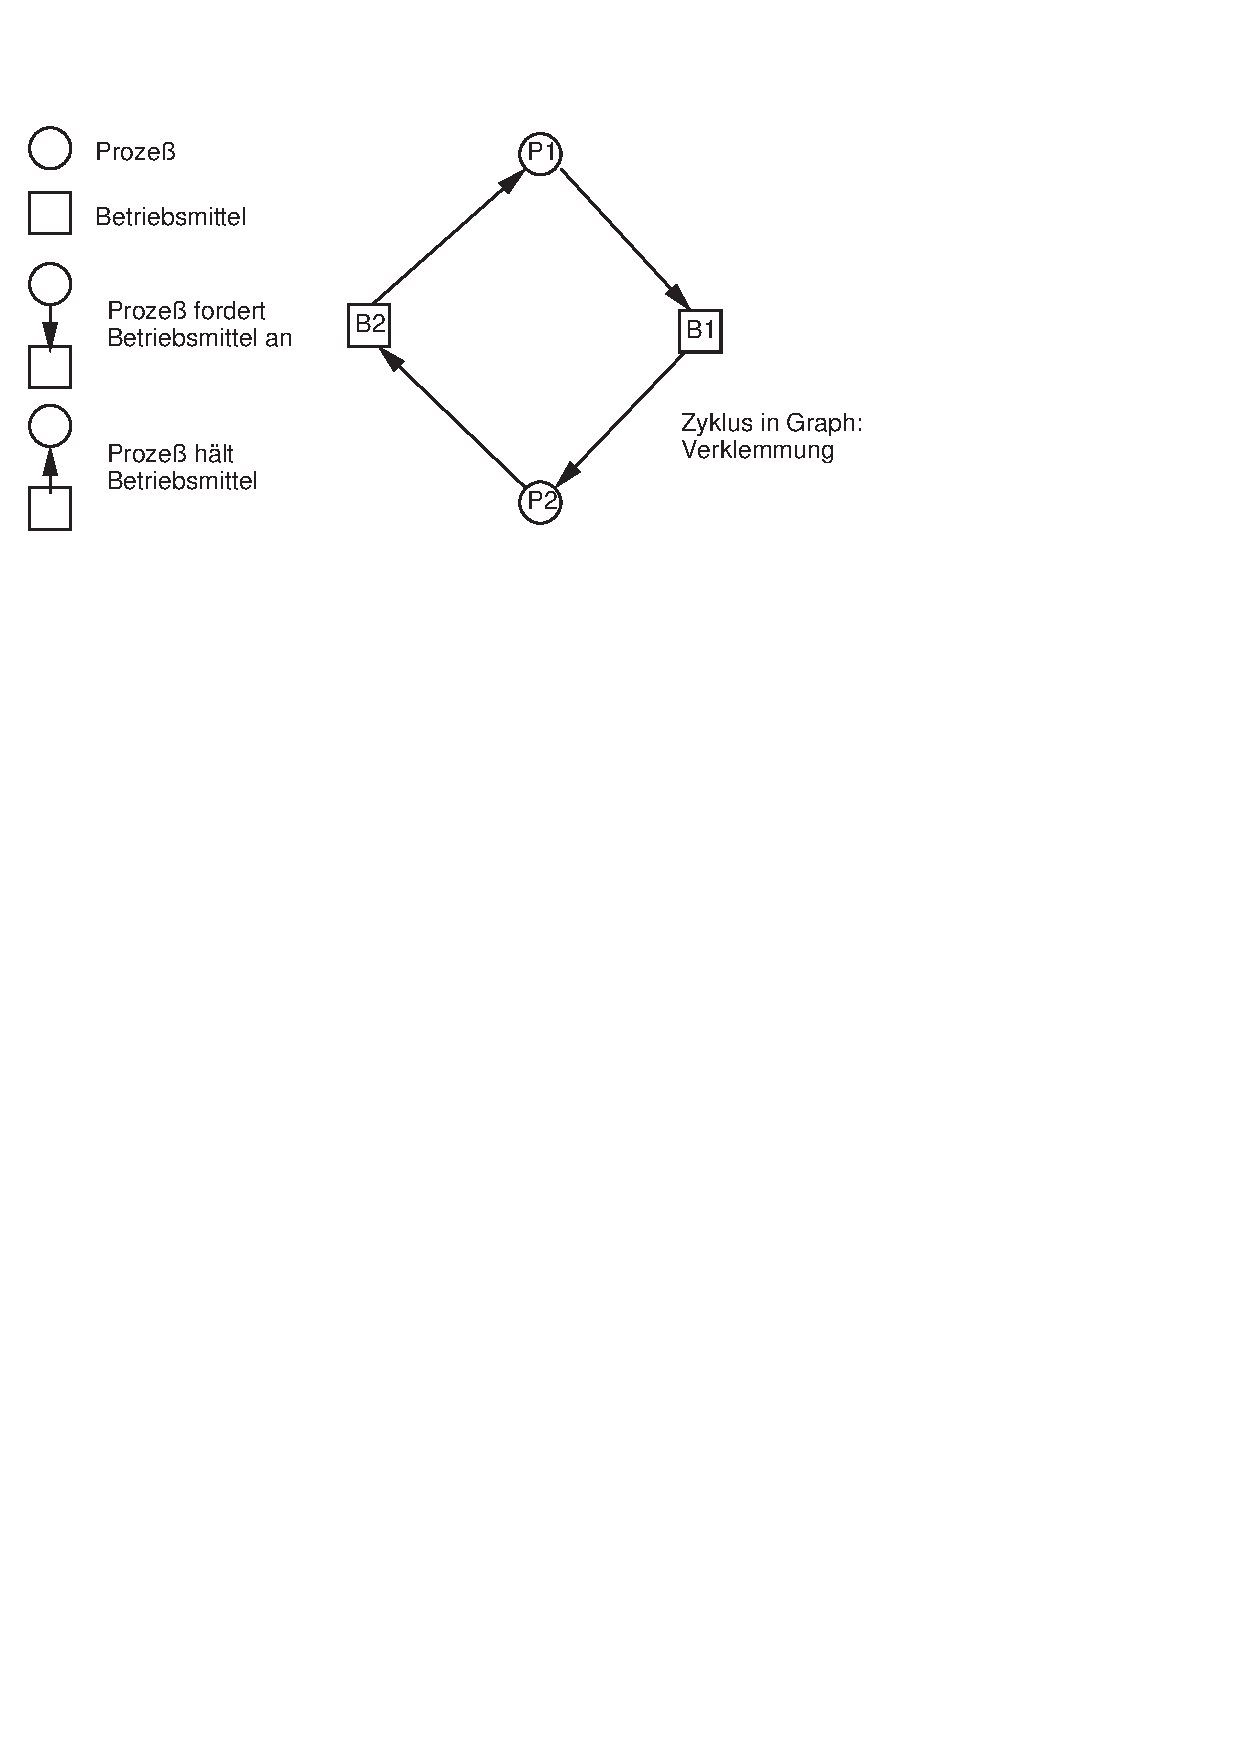
\includegraphics[width=.9\linewidth]{./Abbildungen/deadlock.png}
\end{center}

\subsection*{Vier Strategien mit dem Verklemmungsproblem umzugehen:}
\label{sec:org359aad9}
\begin{itemize}
\item Verklemmungen unmöglich machen
\item Verklemmungen vermeiden
\item Verklemmungen erkennen und beseitigen
\item Verklemmungen ignorieren
\end{itemize}
\subsubsection*{Verklemmungen unmöglich machen}
\label{sec:org97f75e2}
\begin{itemize}
\item Wechselseitigen Ausschluss verhindern (Bedingung 1 ist aufgehoben)
\begin{itemize}
\item Z. B. Einrichten eines Druckerdaemonen
\item Probleme: nicht für alle Betriebsmittel geeignet, nur Verlagerung
auf andere Betriebsmittel
\end{itemize}
\item Zusätzliche Betriebsmittelanforderungen verbieten (Bedingung 2 ist
aufgehoben)
\begin{itemize}
\item Z. B. Anforderung aller benötigten Betriebsmittel zu Prozessbeginn
\item Probleme: Unnötig lange Belegung der Betriebsmittel, schlechte
Betriebsmittelauslastung
\end{itemize}
\end{itemize}
\begin{itemize}
\item Vorzeitige Betriebsmittelrückgabe erzwingbar machen (Bedingung 3 ist
aufgehoben)
\begin{itemize}
\item Z.B. Entzug nach einer bestimmten Zeit
\item Bei CPU selbstverständlich, bei E/A-Geräten meist nicht sinnvoll.
\item Probleme: muss ggf. auf Programmebene berücksichtigt werden,
bereits geleistete Arbeitsleistung geht verloren
\end{itemize}
\item Zirkularität unterbinden (Bedingung 4 ist aufgehoben)
\begin{itemize}
\item Z. B. lineare oder hirarchische Ordnung der Betriebsmittel,
Anforderungen dann nur gemäß dieser Ordnung
\item Probleme: keine allgemein brauchbare Ordnung angebbar, deshalb oft
schlechte Auslastung
\end{itemize}
\end{itemize}
\subsubsection*{Verklemmungsvermeidung}
\label{sec:org9bc4a01}
beruht auf der Grundidee, die Betriebsmittelanforderungen der Prozesse
in eine „verklemmungsfreie” Reihenfolge zu bringen. Die Algorithmen
(Vgl. Bankiersalgorithmus) hierfür sind teiweise sehr komplex und auch
nur anwendbar, wenn der gesamte Betriebsmittelbedarf der Prozesse im
Vorhinein bekannt ist, was in der Praxis häufig nicht der Fall ist.
Nichtsdestotrotz hat sich um dieses Thema herum eine eigene
mathematische Theorie entwickelt, auf die hier aber nicht eingegangen
wird.
\paragraph*{Bankiersalgorithmus}
\label{sec:org8997af0}
\begin{itemize}
\item Betrachtung der Betriebsmittelanforderungen als gleichzeitig
auftretende Maximalforderungen
\item Unterscheidung von
\begin{itemize}
\item \emph{sicheren} Zuständen (Verklemmung nicht möglich)
\item \emph{unsicheren} Zuständen (Verklemmung nicht zwingend, bei
ungünstiger Anforderungsreihen- folge aber möglich)
\end{itemize}
\item Weitere Prozesse werden nur gestartet, wenn kein unsicherer Zustand
entsteht.
\item Auf die Darstellung weiterer Details wird hier verzichtet.
\end{itemize}
\paragraph*{Probleme der Verklemmungsvermeidung}
\label{sec:org9b61d64}
\begin{itemize}
\item I. A. Zahl der maximal benötigten Betriebsmittel unbekannt
\item Ständig wechselnde Zahl von Prozessen
\item Zahl der verfügbaren Betriebsmittel ebenfalls veränderlich
\item Algorithmus ist laufzeit- und speicherintensiv
\end{itemize}
\subsubsection*{Verklemmungen erkennen}
\label{sec:org1790965}
\begin{itemize}
\item Analyse bei verdächtigen Symptomen:
\begin{itemize}
\item viele Prozesse warten und der Prozessor ist unbeschäftigt
\item mindestens zwei Prozesse warten zu lange auf Betriebsmittel
\end{itemize}
\item Bei Verdacht Start eines Erkennungsalgorithmus
\begin{itemize}
\item B. Zyklen-Erkennung im Betriebsmittelgraphen
\end{itemize}
\end{itemize}
\subsubsection*{Verklemmungen beseitigen}
\label{sec:orga2adda9}
\begin{itemize}
\item Prozesse abbrechen
\item Prozesse zurücksetzen
\item Betriebsmittel entziehen
\item Probleme: 
\begin{itemize}
\item Prozess-/Betriebsmittelauswahl
\item Verlust bereits geleisteter Arbeit
\item Mögliche Inkonsistenzen
\item U. U. manueller Mehraufwand erforderlich
\end{itemize}
\end{itemize}
\subsubsection*{Verklemmungen ignorieren}
\label{sec:org822906e}
\begin{itemize}
\item Erkennung von Verklemmungen aufwendig
\item Beseitigung von Verklemmungen nicht unproblematisch
\item Vermeidung bzw. Unmöglichmachen von Verklemmungen u. U. wenig effizient
\item Verklemmungen sind in der Regel nicht das dringlichste Problem
\end{itemize}
\section*{verwendete Literatur}
\label{sec:org904c20a}
\begin{itemize}
\item \cite{Bengel2015}
\item \cite{CACM2017}
\item \cite{CACM2016}
\item \cite{Subramanian2017}
\end{itemize}
\section*{\bibliography{referenzen}}
\label{sec:org2820991}
\end{document}